%%%%%%%%%%%%%%%%%%%%%%%%%%%%%%%%
% Compile with
% pdflatex --shell-escape -synctex=1 -interaction=nonstopmode energyLine.tex
% to convert it to png use:
% convert -density 300 -transparent white energyLine.pdf energyLine.png
%%%%%%%%%%%%%%%%%%%%%%%%%%%%%%%%

\documentclass{standalone}

\usepackage[utf8]{inputenc}
\usepackage{tkz-fct}
\renewcommand{\familydefault}{\sfdefault}
\usepackage[scaled=1]{helvet}
\usepackage[helvet]{sfmath}
\everymath={\sf}
\usetikzlibrary{calc,arrows,intersections,angles,quotes,patterns}

\definecolor{AFLight}{HTML}{5CE0E6}
\definecolor{AFMiddle}{HTML}{51ADE5}
\definecolor{AFDark}{HTML}{0E4160}

\begin{document}

\tikzset{
   name plot/.style={every path/.style={name path global=#1}}
}


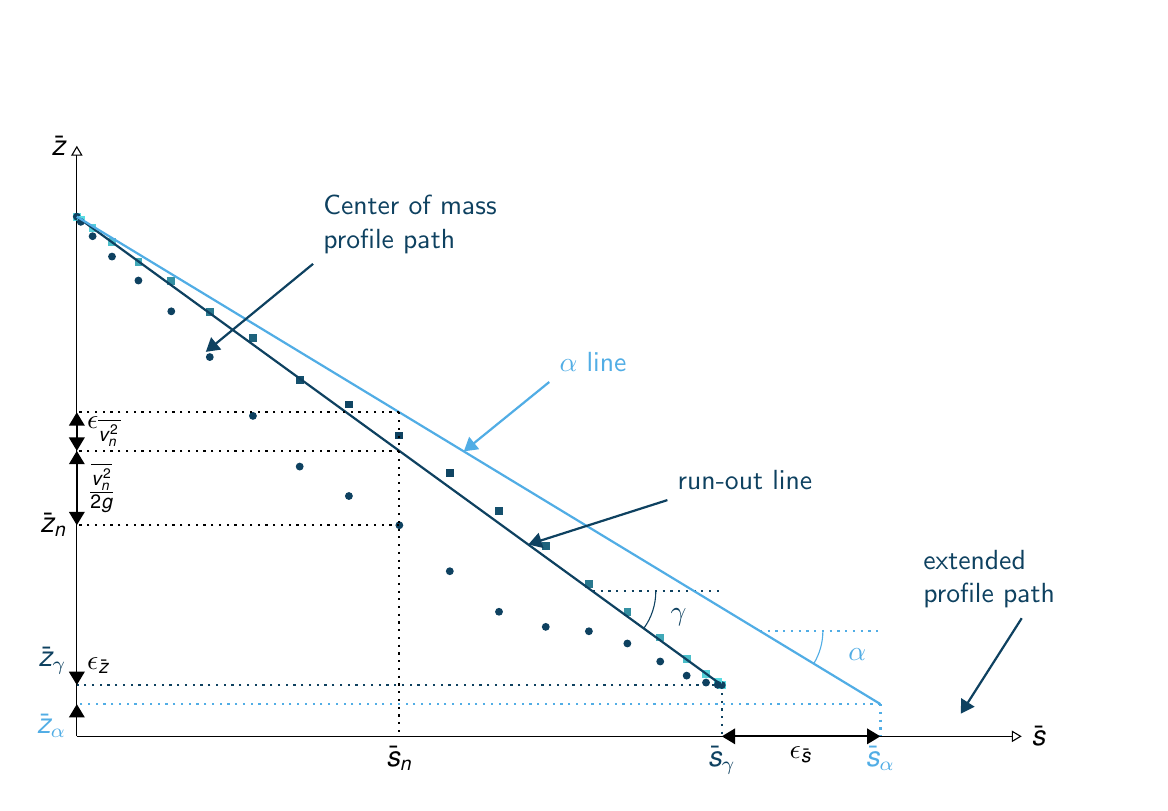
\begin{tikzpicture}[scale=3]


\def\a{0.2222222222}
\def\b{-1.3333}
\def\c{2.2}

\def\aa{0.215}
\def\bb{-1.38}
\def\cc{3.15}
\def\alp{-30}
\def\gam{-36}
\def\sincoef{0.1}

\pgfmathsetmacro\sinprop{9.5*180/3.14}

% center of mass path end
\pgfmathsetmacro\xa{(tan(\gam)-\b)/\a}
\pgfmathsetmacro\ya{\a*\xa*\xa+\b*\xa+\c+\sincoef*sin(\sinprop)*sin(\sinprop)}

% run out line angle
\pgfmathsetmacro\xai{0.8*\xa}
\pgfmathsetmacro\yai{\c-(\c-\ya)/\xa*\xai}
\pgfmathsetmacro\yaii{\a*\xa*\xa+\b*\xa+\c+\sincoef*sin(\sinprop)*sin(\sinprop)}
\pgfmathsetmacro\xao{1*\xa}
\pgfmathsetmacro\yao{\yai}

% alpha line angle
\pgfmathsetmacro\xaa{(tan(\alp)-\b)/\a}
\pgfmathsetmacro\yaa{\ya+(2*\a*\xa+\b)*(\xaa-\xa)}
\pgfmathsetmacro\xaai{0.85*\xaa}
\pgfmathsetmacro\yaai{\c-(\c-\yaa)/\xaa*\xaai}
\pgfmathsetmacro\xaao{1*\xaa}
\pgfmathsetmacro\yaao{\yaai}


% center of mass path name
\pgfmathsetmacro\xp{0.2*\xa}
\pgfmathsetmacro\yp{\a*\xp*\xp+\b*\xp+\c+\sincoef*sin(\xp/\xa*\sinprop)*sin(\xp/\xa*\sinprop}
% alpha line name
\pgfmathsetmacro\xal{0.6*\xa}
\pgfmathsetmacro\yal{\c-(\c-\yaa)/\xaa*\xal}
% gamma line name
\pgfmathsetmacro\xg{0.7*\xa}
\pgfmathsetmacro\yg{\c-(\c-\yai)/\xai*\xg}
% extended profile name
\pgfmathsetmacro\xep{1.1*\xaa}
\pgfmathsetmacro\yep{\ya+(2*\a*\xa+\b)*(\xep-\xa)}

% point somewhere on the way
\pgfmathsetmacro\xb{0.5*\xa}
\pgfmathsetmacro\yb{\a*\xb*\xb+\b*\xb+\c+\sincoef*sin(\xb/\xa*\sinprop)*sin(\xb/\xa*\sinprop)}
\pgfmathsetmacro\ybi{\c-(\c-\ya)/\xa*\xb}
\pgfmathsetmacro\ybii{\c-(\c-\yaa)/\xaa*\xb}

\tkzInit[xmin=0,xmax=4.5,ymin=0,ymax=3]
% Draw coordinates
\draw [>={Triangle[open]},thin, ->] (0,0) --  (0,2.5) node[left] {$\bar{z}$};
\draw[>={Triangle[open]},thin, ->]  (0,0) --  (4,0) node[right] {$\bar{s}$};
% Draw center of mass path line and points
\tkzFct[thick,color=AFDark,domain=0:\xa]{(\a*x*x+\b*x+\c+\sincoef*sin(x/\xa*\sinprop*3.14/180)*sin(x/\xa*\sinprop*3.14/180))}
\tkzFct[thick, dotted, color=AFDark,domain=\xa:4]{\ya+(2*\a*\xa+\b)*(x-\xa)}

\foreach \i in {0.0,0.05,...,1.1} {
    \pgfmathsetmacro{\j}{(1-sin(\i*180)*sin(\i*180))*100}
    \pgfmathsetmacro{\xx}{(-0.5*cos(\i*180) + 0.5 )*\xa}
    \pgfmathsetmacro{\yy}{\c-(\c-\ya)/\xa*\xx + (rand - 0.5)*0.05*(cos(\i*180)*cos(\i*180)-1)}
    \pgfmathsetmacro{\yyy}{(\sincoef*sin(\xx/\xa*\sinprop)*sin(\xx/\xa*\sinprop) + \a*\xx*\xx+\b*\xx+\c)}

   \draw [color=AFLight!\j!AFDark] plot [only marks, mark size=0.4, mark=square*] coordinates {(\xx, \yy)};
   \draw [color=AFDark] plot [only marks, mark size=0.4, mark=*] coordinates {(\xx, \yyy)};
}

\tkzDefPoints{0/\c/H, \xa/0/A, \xa/\ya/AA, 0/\ya/AAA, \xai/\yai/AI, \xao/\yao/AO, \xp/\yp/P, \xaa/0/A1, \xaa/\yaa/AA1, 0/\yaa/AAA1, \xaai/\yaai/AI1, \xaao/\yaao/AO1, \xb/\yb/B, 0/\yb/BB, \xb/0/B0, \xb/\ybi/BI1, 0/\ybi/BI2, \xb/\ybii/BII1, 0/\ybii/BII2, \xg/\yg/G, \xal/\yal/AL, \xep/\yep/EP}
% gamma line/ run out line
\draw [thick,dotted, AFDark] (AA) -- (A) node [below] {$\bar{s}_{\gamma}$};
\draw [thick,dotted, AFDark] (AA) -- (AAA) node [above left] {$\bar{z}_{\gamma}$};
\draw [thick, AFDark] (AA) -- (H);
\draw [thick,dotted, AFDark] (AI) -- (AO);
\pic[draw,AFDark,angle radius=0.8cm,"$\gamma$" ,pic text options={shift={(18pt,-5pt)}}]{angle=AA--AI--AO};
% alpha line
\draw [thick,dotted, AFMiddle] (AA1) -- (A1) node [below] {$\bar{s}_{\alpha}$};
\draw [thick,dotted, AFMiddle] (AA1) -- (AAA1) node [below left] {$\bar{z}_{\alpha}$};
\draw [thick,thick, AFMiddle] (AA1) -- (H);
\draw [thick,dotted, AFMiddle] (AI1) -- (AO1);
\pic[draw,AFMiddle,angle radius=0.8cm,"$\alpha$" ,pic text options={shift={(22pt,-5pt)}}]{angle=AA1--AI1--AO1};

% some point on the way
\draw [thick,dotted, black] (BII1) -- (B0) node [below] {$\bar{s}_{n}$};
\draw [thick,dotted, black] (B) -- (BB) node [left] {$\bar{z}_{n}$};
\draw [thick,dotted, black] (BI1) -- (BI2) node [below] {};
\draw [thick,dotted, black] (BII1) -- (BII2) node [below] {};


\draw [>={Triangle},thick, <->] (BB) -- (BI2) node [midway,right,black] {$\frac{\overline{v^2_n}}{2g}$};
\draw [>={Triangle},thick, <->] (BI2) -- (BII2) node [midway,right,black] {$\epsilon_{\overline{v^2_n}}$};
\draw [>={Triangle},thick, <->] (A) -- (A1) node [midway,below,black] {$\epsilon_{\bar{s}}$};
\draw [>={Triangle},thick, ->] (AAA) + (0,0.01) -- (AAA) node [midway,above right,black] {$\epsilon_{\bar{z}}$};
\draw [>={Triangle},thick, ->] (AAA1) + (0,-0.01) -- (AAA1) node [black] {};


\node[text width=2.5cm, fill=none,above right,AFDark] at (1,2) {Center of mass\\ profile path};
\draw [>={Triangle},thick, ->, AFDark] (1,2) -- (P);
\node[text width=2.5cm, fill=none,above right,AFMiddle] at (2,1.5) {$\alpha$ line};
\draw [>={Triangle},thick, ->, AFMiddle] (2,1.5) -- (AL);
\node[text width=2.5cm, fill=none,above right,AFDark] at (2.5,1) {run-out line};
\draw [>={Triangle},thick, ->, AFDark] (2.5,1) -- (G);
\node[text width=2.5cm, fill=none,above,AFDark] at (4,0.5) {extended\\profile path};
\draw [>={Triangle},thick, ->, AFDark] (4,0.5) -- (EP);
\end{tikzpicture}

\end{document}
